%===================================== CHAP 1 =================================

\chapter{Introduction}

\section{Motivation}
Automated motion control of ships has been a topic of extensive research in the last 60 years. In moving from simple course-keeping assistant systems on traditional manned vessels, to fully automated unmanned autonomous vessels, the need for more efficient and sophisticated control systems has grown. In recent years, the research has expanded from control of manned vessels to also include unmanned vessels. Challenges include handling uncertain nonlinear hydrodynamics and external disturbances, since the ocean is an unreliable environment with non-linearities and unpredictable perturbations. Hence, it is important to develop adaptive and robust control algorithms, which can deal with these internal uncertainties and external disturbances in a realistic and energy efficient manner. It is also important to
consider physical magnitude and rate saturation constraints for the actuators.


\section{Problem formulation}



\section{Literature}
\subsection{$\mathcal{L}_1$ Adaptive control}
The term $\mathcal{L}_1$ Adaptive control was coined and the underlying control method was first developed by Chengyu Cao and Naira Hovakimyan \citep{Cao20061}-\citep{Cao20062}. The name originates from the concept of the $\mathcal{L}_1$ norm needed to prove stability of the control law. One of the key features of this control concept compared to other adaptive approaches is the decoupling of the adaptation loop and the control loop, allowing fast adaptation. 

The high-gain $\mathcal{L}_1$ adaptive approach was proposed as a way to address the inherent uncertainties that is present in most kinematic models. The fast adaptation property has been extensively utilized for vessels in marine applications, such as a high-speed personal watercraft(PWC) in \cite{Casper} and aerial application as \cite{L1aircraft}. The high-gain $\mathcal{L}_1$ adaptive scheme has shown usefulness in such application, being capable of handling sudden changes in disturbance and large model uncertainties. 
\begin{figure}[!h]
    \centering
    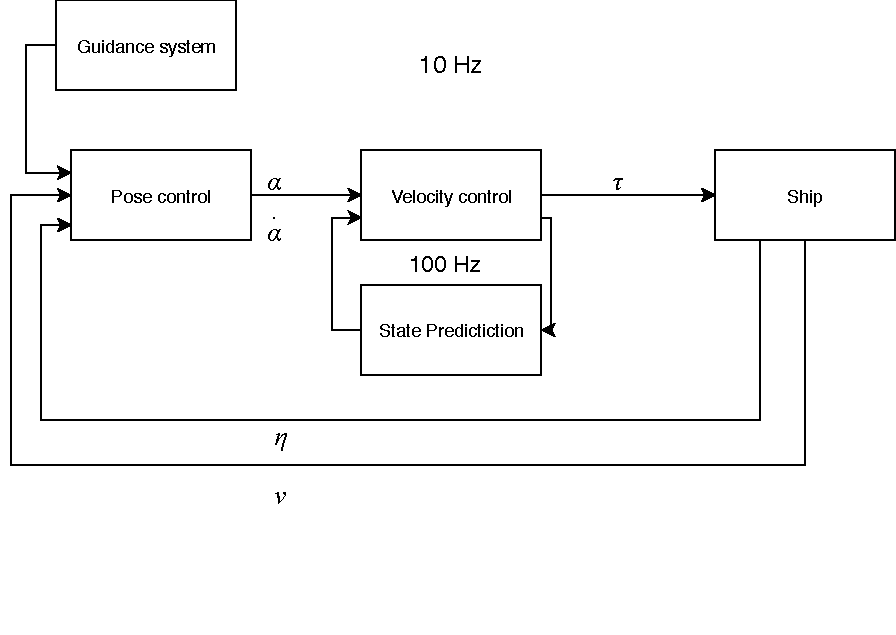
\includegraphics[width=0.75\textwidth]{fig/L1diagram}
    \caption{Principal sketch of the $\mathcal{L}_1$ Adaptive architecture used in this thesis}
    \label{fig:L1sketch}
\end{figure}

Fig. \ref{fig:L1sketch} shows the concept of the $\mathcal{L}_1$ architecture applied on a cascaded control structure, as used in this thesis. The decoupling of control and adaptation is shown, where the state prediction runs at 100 Hz while the control system runs at 10 Hz. This concept is shown in Fig. \ref{fig:L1pred}, for the pose state $\boldsymbol{\eta}$. At every 10 samples, a new measurement is given to the controller as seen in Fig. \ref{fig:L1sketch}, and in between samples the state is predicted. This is done for both velocity and position. 

\begin{figure}[!h]
    \centering
    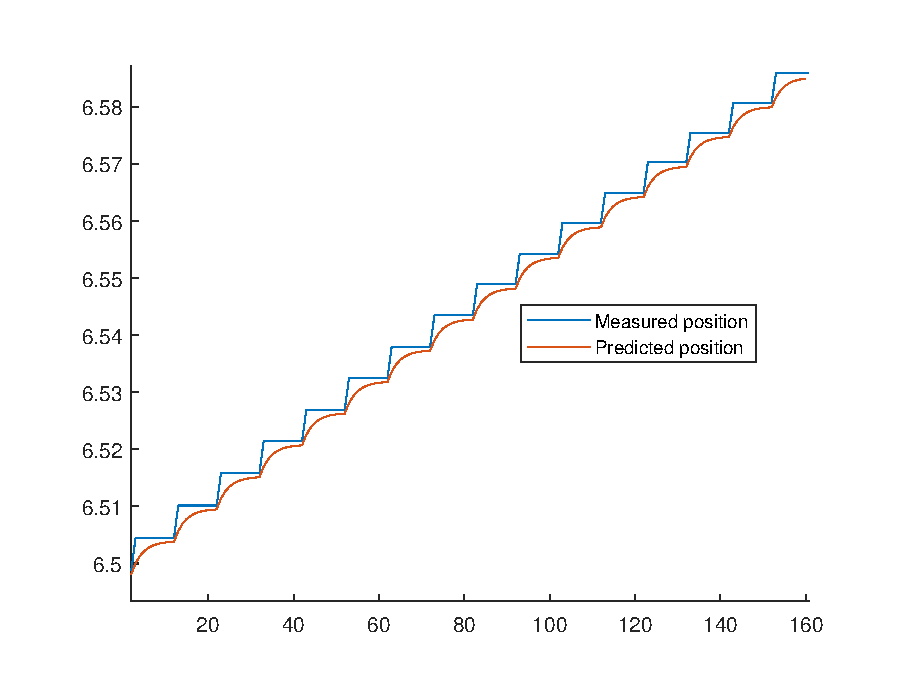
\includegraphics[width=0.75\textwidth]{fig/L1statepred.eps}
    \caption{State prediction in $\mathcal{L}_1$ adaptive control}
    \label{fig:L1pred}
\end{figure}


\newpage
\subsection{Command Governor}


Command governor-based control is an approach for augmenting the tracking signal given to the control system, in order to improve the tracking signal. The core idea behind using command governor can be conceptually compared to using a reference model for introducing input reference to the control system. In case of a rapid change/step in the desired pose, the reference will smoothe the input signal to avoid saturation. Similarly, the motivation behind command governor is to achieve predicable transient and tracking behaviour of a closed-loop control system, without resorting to a high-gain adaption scheme. \\A novel command governor architecture is proposed in \cite{CommandGov}, and proven to cause the closed-loop system to approximate a Hurwitz LTI system, and stabilizing the uncertain, nonlinear model to Lyapunov. \\ More specifically, what the command governor idea is trying to do is to avoid the need for knowledge of the specific, conservative upper bound on the unknown weights in the uncertainty parametrization of the model, which might not be feasible to find in all applications. Without knowing the bound, it is difficult to design controllers that achieve predictable transient response and steady-state of the closed-loop.

In further literature, in \cite{CommandGov2}, the command governor adaptive architecture is applied to a 6 degrees-of-freedom autonomous helicopter, and achieved improved tracking results using the command governor compared to the baseline adaptive control. 

\begin{figure}[!h]
    \centering
    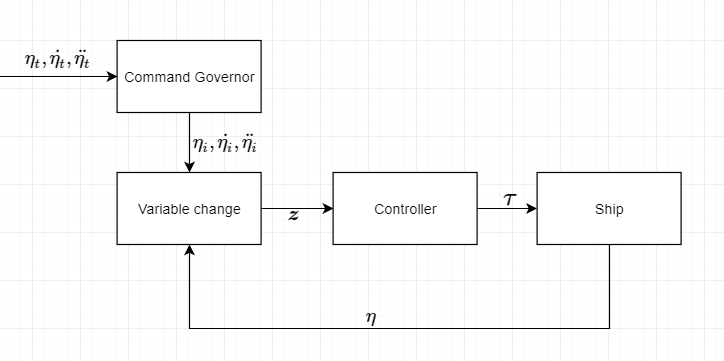
\includegraphics[width=0.78\textwidth]{fig/CGconcept.png}
    \caption{Principal sketch of the Command Governor architecture}
    \label{fig:CGsketch}
\end{figure}

\subsection{Magnitude-Rate Saturation - MRS}


\begin{figure}[!h]
    \centering
    \begin{tikzpicture}[auto, node distance=1.5cm,>=latex']
    \node [input, name=input1] (input1) {};
    \node [block, right of=input1,minimum size=0.8cm] (der) {$s$};
    \node [sum, right of=der] (sum1) {};
    \node [satblock, right of=sum1,minimum size=0.8cm] (satblock1) {};
    \node [block, right of=satblock1,minimum size=0.8cm] (int) {$\frac{1}{s}$};
    \node [satblock, right of=int,minimum size=0.8cm] (satblock2) {};
    \node [output, right of=satblock2,minimum size=0.8cm] (output1) {};
    \node [block, above of=sum1,minimum size=0.8cm] (K) {$\boldsymbol{K}$};
    \node [sum, above of=K] (sum2) {};
    \node [tmp, right of=sum2] (tmp1){};
    \node [tmp, left of=sum2] (tmp2){};
    
    \draw [->] (input1) -- node[name=x,anchor=north]{} (der);
    \draw [->] (der) -- node[anchor=north]{$+$} (sum1);
    \draw [->] (K) -- node[anchor=east, pos=0.95]{$+$} (sum1);
    \draw [->] (sum2) -- (K);
    \draw [->] (sum1) -- (satblock1);
    \draw [->] (satblock1) -- node{$\dot{\boldsymbol{\delta}}$}(int);
    \draw [->] (int) -- node{$\boldsymbol{\delta}$}(satblock2);
    \draw [->] (input1) -- node[anchor=north]{$\boldsymbol{\tau}_c$} (der);
    \draw [->] (satblock2) -- node [name=y,anchor=north]{$\boldsymbol{\tau}_{mrs}$} (output1);
    \draw [->] (y) |- (tmp1) |- node[pos=0.95,anchor=south]{$-$} (sum2);
    \draw [->] (x) |- (tmp2) |- node[pos=0.95]{$+$} (sum2);
    
    \end{tikzpicture}
    \caption{Diagram of an MRS model. From \cite{}}
    \label{fig:blockdiagram_MRS}
\end{figure}

\subsection{Immersion and Invariance}

Immersion and Invariance, I\&I, as phrased in \cite{II2003} is an approach for adaptive control of nonlinear systems, as well as stabilization. The approach aims to reduce the problem of designing a control system capable of adaptive stabilization of a nonlinear system into sub-problems, which can be easier to solve. This approach can be a solution in design situations where, using traditional nonlinear design, one should find a appropriate Lyapunov function candidate, which might not always be feasible. 

\todo{Expand on this paragraph}

\section{Contributions}

The main contributions from this thesis are.


\section{Outline}
This thesis is composed of 6 chapters: Chapter 1 gives an introduction to the subject and technologies used; Chapter 2 details the deriving of the ship maneuvering model and the control approach; Chapter 3 explains the simulation setup and results of the control approaches; Chapter 4 presents the Marine Cybernetics Laboratory(MC-lab) and the results from lab experiments from scale-model testing, as well as modifications done between lab sessions; Chapter 5 is analysis and discussion of results; while Chapter 6 concludes the thesis and proposes further work. 


\cleardoublepage